\documentclass[12pt]{article}
\usepackage[letterpaper, total={6in, 8in}]{geometry}
\setlength{\oddsidemargin}{0in}
\setlength{\evensidemargin}{0in}
\setlength{\textwidth}{6.5in}
\setlength{\parindent}{0in}
\setlength{\parskip}{\baselineskip}

\usepackage{amsmath,amsfonts,amssymb}
\usepackage{subfigure}
\usepackage{sectsty}
\usepackage{multirow}
\usepackage{makecell}
\usepackage{float}
\usepackage[utf8x]{inputenc}
\usepackage[pdftex]{graphicx}
\usepackage[toc,page]{appendix}
\usepackage{enumitem}
\usepackage{indentfirst}
\usepackage{scrextend}
\usepackage{caption}
\usepackage{hyperref}

\usepackage{listings}
\usepackage{color} %red, green, blue, yellow, cyan, magenta, black, white
\definecolor{mygreen}{RGB}{28,172,0} % color values Red, Green, Blue
\definecolor{mylilas}{RGB}{170,55,241}

\DeclareFixedFont{\ttb}{T1}{txtt}{bx}{n}{10} % for bold
\DeclareFixedFont{\ttm}{T1}{txtt}{m}{n}{10}  % for normal

\usepackage{color}
\definecolor{deepblue}{rgb}{0,0,0.5}
\definecolor{deepred}{rgb}{0.6,0,0}
\definecolor{deepgreen}{rgb}{0,0.5,0}

\usepackage{listings}
\lstset{language=Matlab,%
	%basicstyle=\color{red},
	breaklines=true,%
	morekeywords={matlab2tikz},
	keywordstyle=\color{blue},%
	morekeywords=[2]{1}, keywordstyle=[2]{\color{black}},
	identifierstyle=\color{black},%
	stringstyle=\color{mylilas},
	commentstyle=\color{mygreen},%
	showstringspaces=false,%without this there will be a symbol in the places where there is a space
	numbers=left,%
	numberstyle={\tiny \color{black}},% size of the numbers
	numbersep=9pt, % this defines how far the numbers are from the text
	emph=[1]{for,end,break},emphstyle=[1]\color{red}, %some words to emphasise
	%emph=[2]{word1,word2}, emphstyle=[2]{style},    
}


% Python style for highlighting
\newcommand\pythonstyle{\lstset{
		language=Python,
		basicstyle=\ttm,
		otherkeywords={self},             % Add keywords here
		keywordstyle=\ttb\color{deepblue},
		emph={MyClass,__init__},          % Custom highlighting
		emphstyle=\ttb\color{deepred},    % Custom highlighting style
		stringstyle=\color{deepgreen},
		frame=tb,                         % Any extra options here
		showstringspaces=false            % 
}}


% Python environment
\lstnewenvironment{python}[1][]
{
	\pythonstyle
	\lstset{#1}
}
{}

% Python for external files
\newcommand\pythonexternal[2][]{{
		\pythonstyle
		\lstinputlisting[#1]{#2}}}

% Python for inline
\newcommand\pythoninline[1]{{\pythonstyle\lstinline!#1!}}

\begin{document}
\hfill Sam Feig $|$ Vladimir Zhdanov \\
\textbf{H3}\hfill CSCI 4831/5722 \\
\rule{\textwidth}{.75pt}

\begin{enumerate}
	\item 
	\begin{enumerate}
		\item This proof will be shown for the $3*3$ kernel size but is the same for any $k > 1$. Consider the following separable 2D filter kernel $g$ of size $2k + 1$ with $k = 1$.
		\begin{align*}
		g_1 &= \begin{bmatrix} w_4 & w_5 & w_6 \end{bmatrix} \\
		g_2 &= \begin{bmatrix} w_1 \\ w_2 \\ w_3 \end{bmatrix} \\
		g &= g_2g_1 \\  
		&= \begin{bmatrix}
		w_1w_4 & w_1w_5 & w_1w_6 \\
		w_2w_4 & w_2w_5 & w_2w_6 \\
		w_3w_4 & w_3w_5 & w_3w_6 
		\end{bmatrix}
		\end{align*}
		Then, consider the following value for our "image" $f$, where the pixel of interest for this proof is $x$.
		\begin{align*}
		f &= \begin{bmatrix}
		a_1 & a_2 & a_3 \\
		a_4 & x & a_5 \\
		a_6 & a_7 & a_8 
		\end{bmatrix}
		\end{align*}
		
		Then, the convolution of $f$ with $g$ on the pixel $x$ is:
		\begin{align*}
		h_{2D}(m, n) &= \sum_{k, l} g(k, l) f(m + k, n + l) \\
		&= a_1w_1w_4 + a_2w_1w_5 + a_3w_1w_6 + a_4w_2w_4 + \\ &xw_2w_5 + a_5w_2w_6 + a_6w_3w_4 + a_7w_3w_5 + a_8w_3w_6
		\end{align*}
		
		Now, we must confirm that applying each of the 1D convolutions separately gives the same result. The convolution of $f$ with $g_1$ is:
		\begin{align*}
		h_1 &= \sum_l g_1(l) f(m, n+l) \\
		&= \begin{bmatrix}
		w_4a_1 + w_5a_2 + w_6a_3 \\
		w_4a_4 + w_5x + w_6a_5 \\
		w_4a_6 + w_5a_7 + w_6a_8
		\end{bmatrix}
		\end{align*}
		Then, the convolution of $h_1$ (the result from the previous step) with $g_2$ gives the following.
		\begin{align*}
		h_2 &= \sum_k g_2(k) h_1(m + k) \\
		&= a_1w_1w_4 + a_2w_1w_5 + a_3w_1w_6 + a_4w_2w_4 + \\ &xw_2w_5 + a_5w_2w_6 + a_6w_3w_4 + a_7w_3w_5 + a_8w_3w_6
		\end{align*}
		Thus, the result is the same in both cases, so convolving an image with a discrete, separable 2D filter kernel is equivalent to convolving with two 1D filter kernels.
		
		\item For each pixel, a 2D filter kernel would perform $(2k + 1)^2$ operations, while each 1D filter kernel would perform $2k + 1$ operations. So, the number of operations saved per pixel is:
		\begin{align*}
		(2k +1) ^2 - 2 * (2k + 1) &= (4k^2 + 4k + 1) - (4k + 2) \\
		&= 4k^2 - 1
		\end{align*}
		Based on this, the total number of operations saved for an $N*N$ image is $\boxed{N^2(4k^2 - 1)}$.
	\end{enumerate}





	\item 
	\item
	\item
	\item A way to verify that repeatedly applying an averaging filter will approximate Gaussian smoothing is to take an image and apply both side by side. First, apply a Gaussian smooth to it, then take the original image and apply a averaging filter with a small kernel size like 3x3. Then repeat the application of the averaging filter until the output image looks approximately like the result of the Gaussian smoothing. Then, if we take the root mean square error of the pixels for both images compared to the original image and take the average of their difference, we can have an average RMS error for the difference between Gaussian smoothing and repeated averaging. As you can see from the plot below, the error is very small meaning the Gaussian smoothing with sigma=2 and using a 3x3 averaging filter 5 times are very close to the same effect. \\
	\begin{centering}
		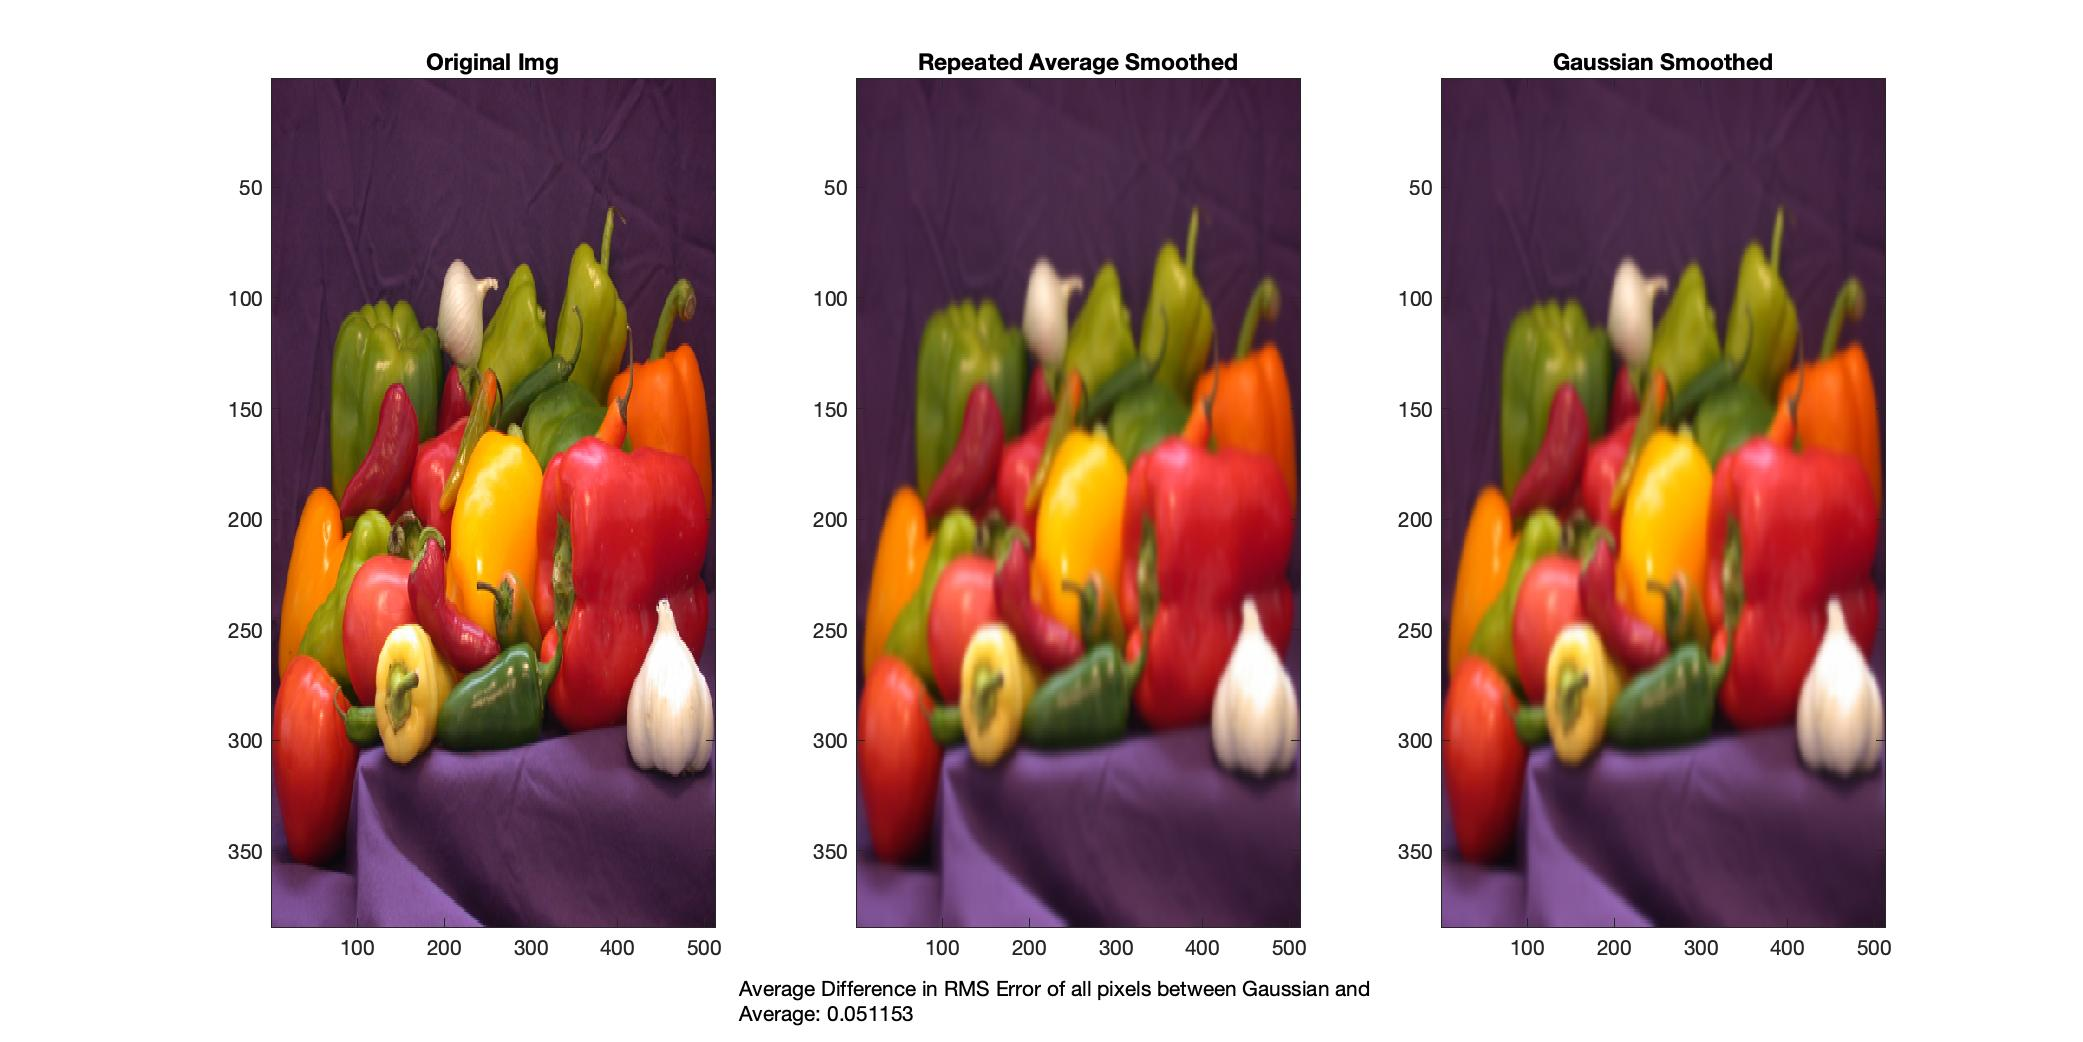
\includegraphics[width=1\textwidth]{Q5_results.jpg}
	\end{centering}
	
	\item
	\begin{enumerate}
		\item text
		
		\begin{centering}
			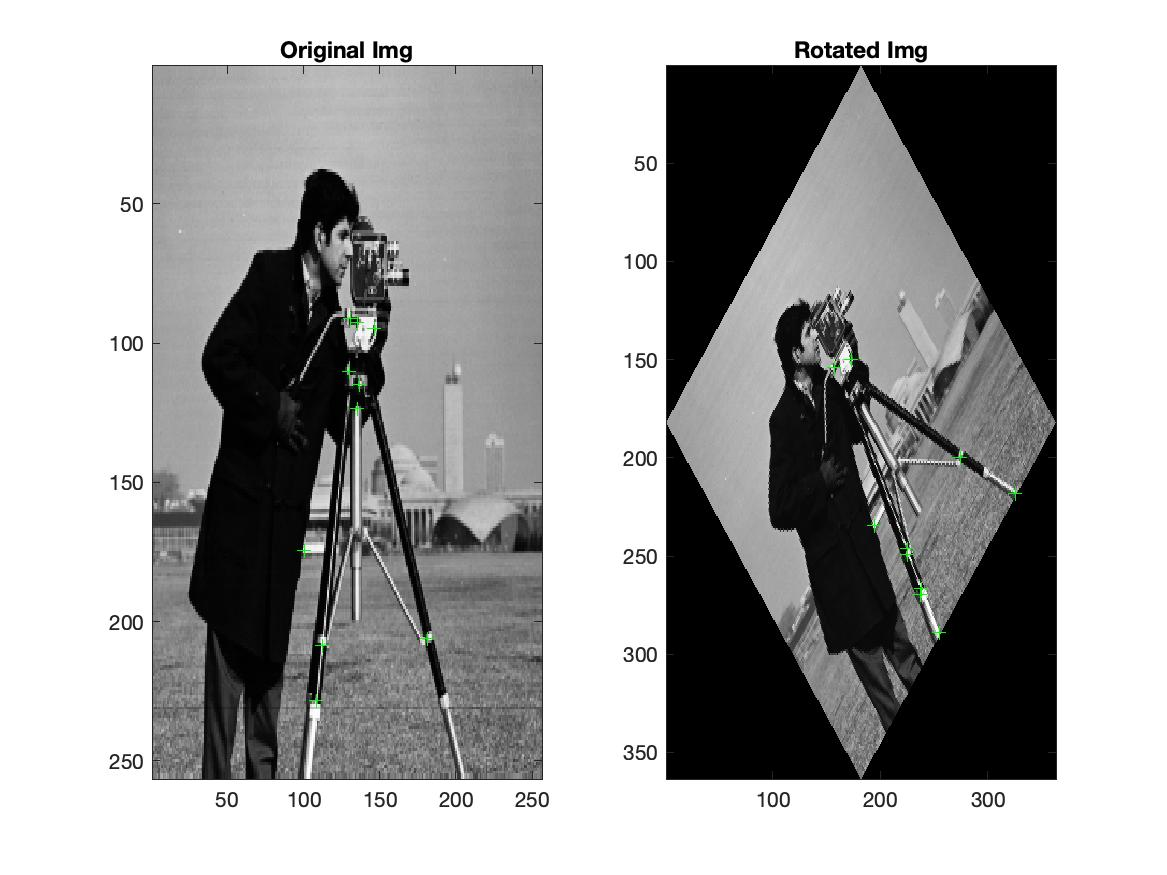
\includegraphics[width=0.5\textwidth]{Q6A_rot_results.jpg}
			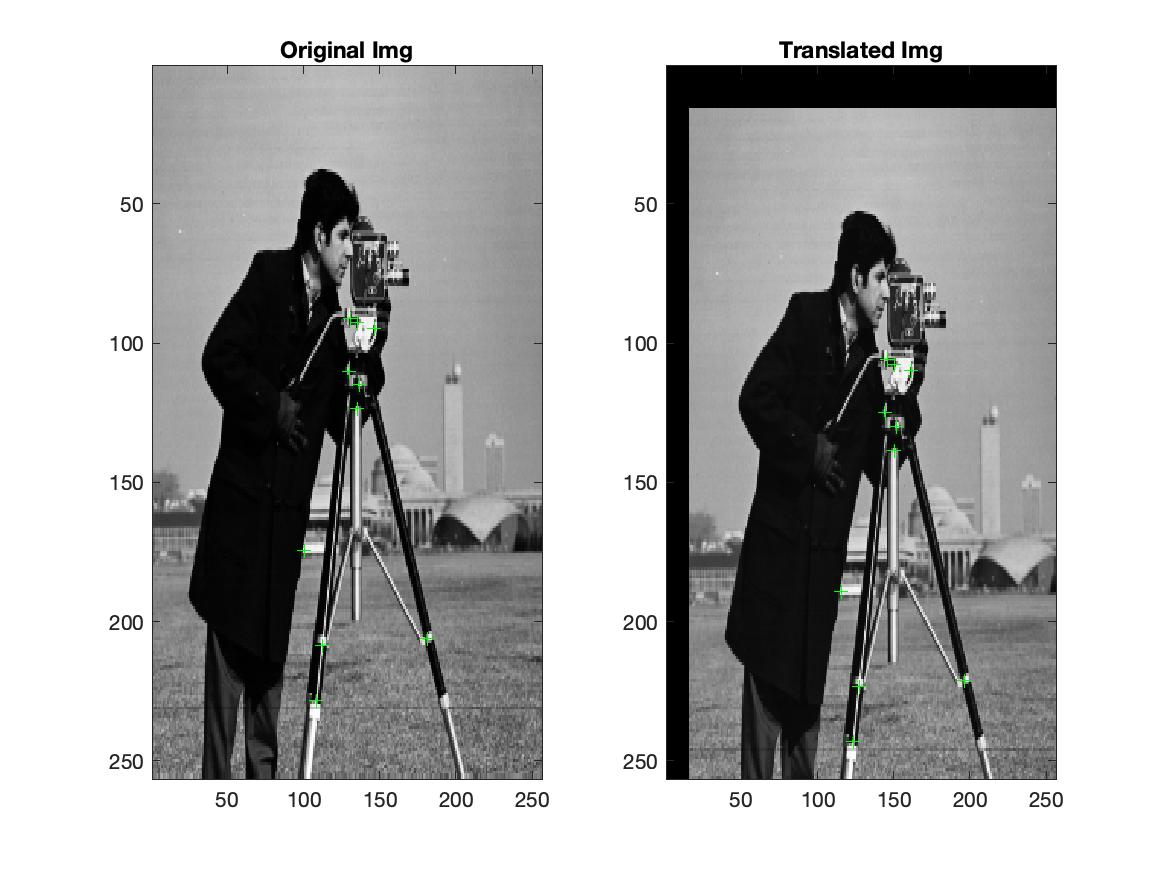
\includegraphics[width=0.5\textwidth]{Q6A_trans_results.jpg}
			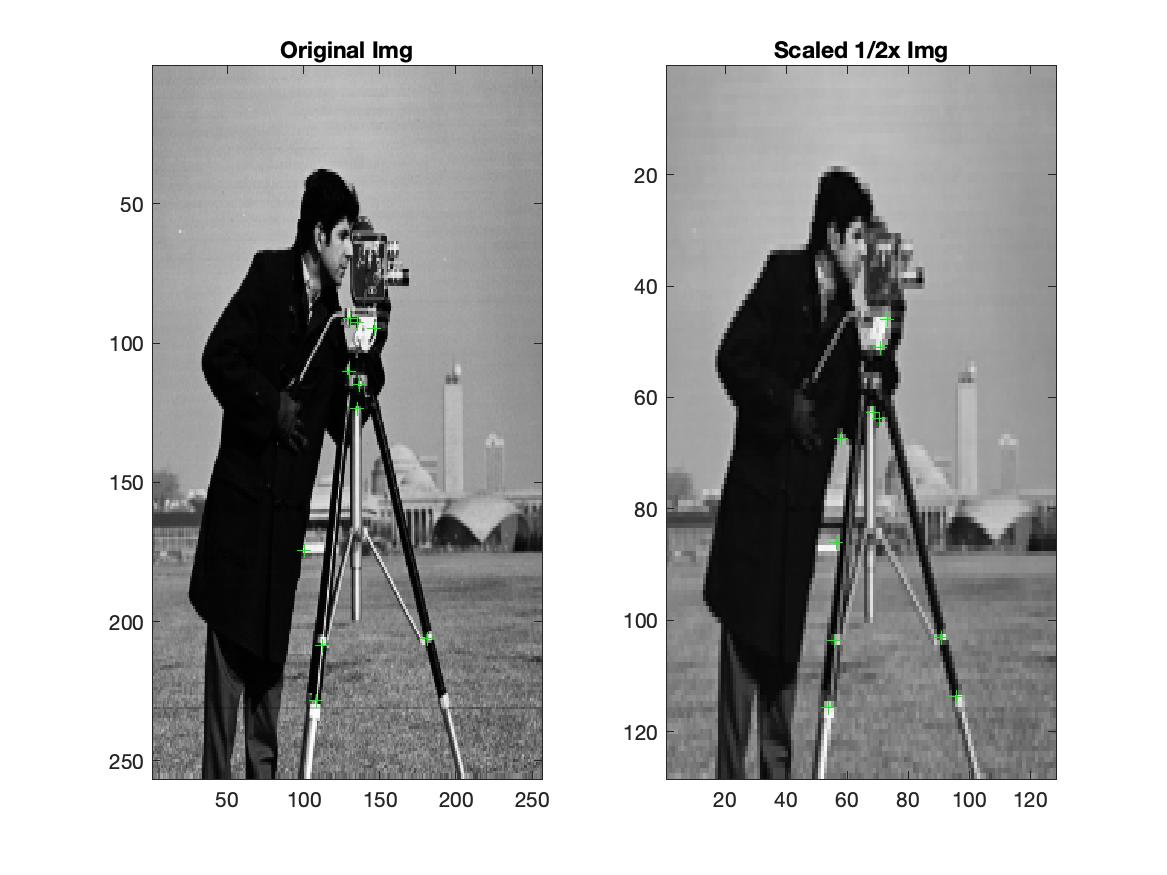
\includegraphics[width=0.5\textwidth]{Q6A_scale_results.jpg}
			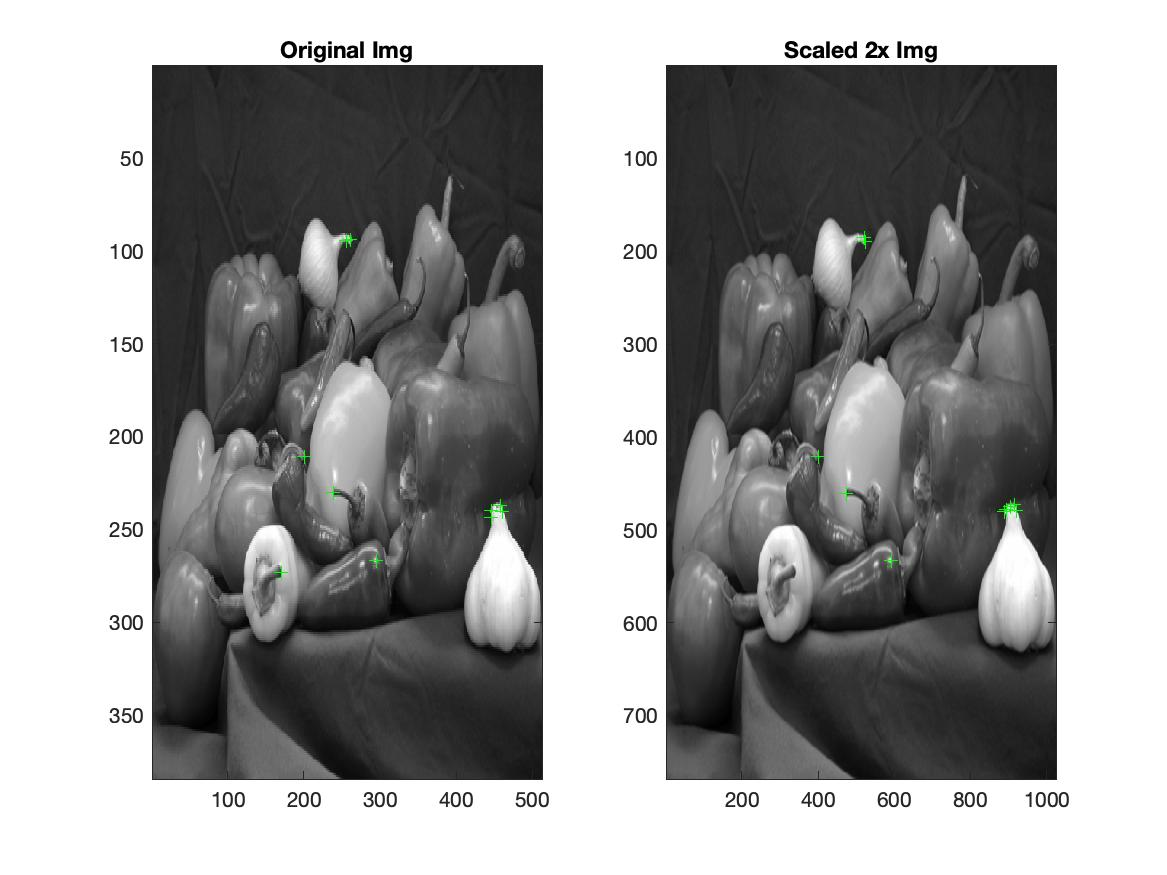
\includegraphics[width=0.5\textwidth]{Q6A_scale2_results.jpg}
		\end{centering}
		
		\item text2
		
		\begin{centering}
			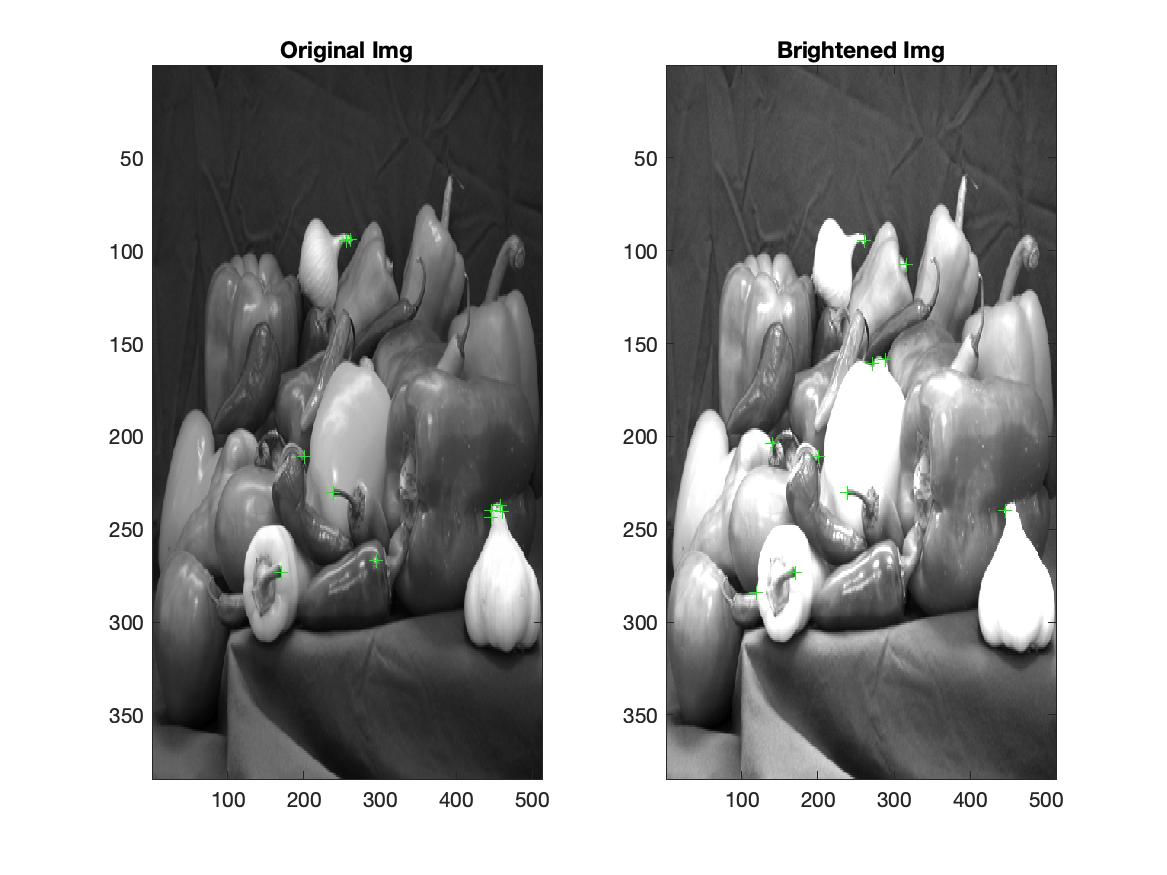
\includegraphics[width=0.5\textwidth]{Q6B_bright_results.jpg}
			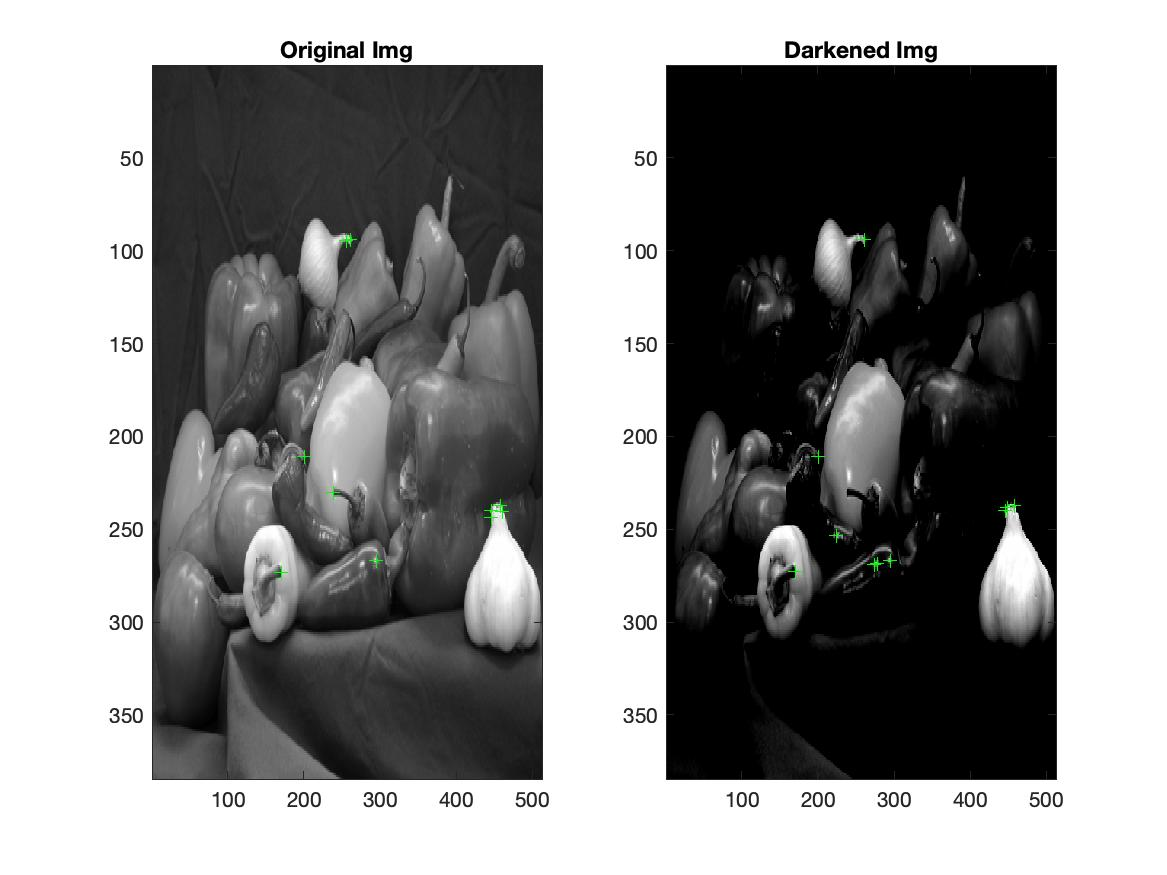
\includegraphics[width=0.5\textwidth]{Q6B_dark_results.jpg}
			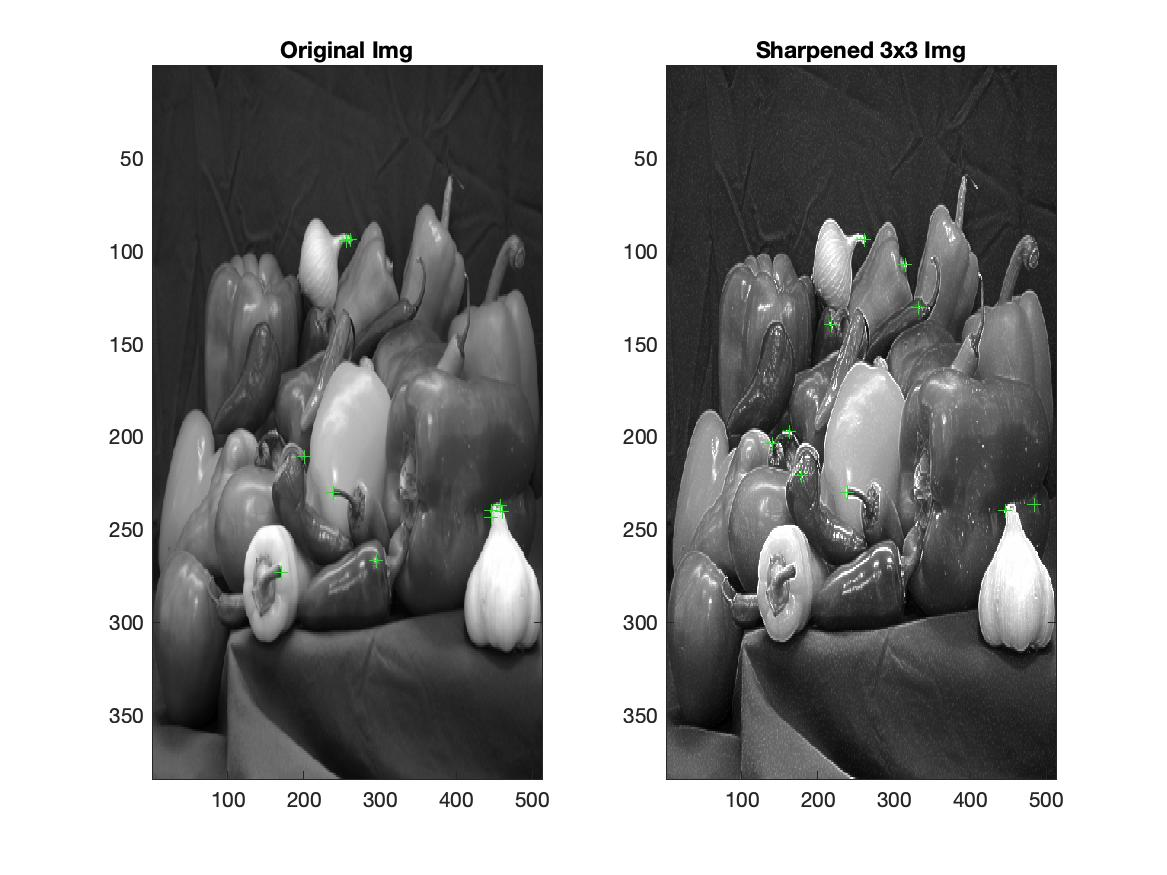
\includegraphics[width=0.5\textwidth]{Q6B_sharp3_results.jpg}
			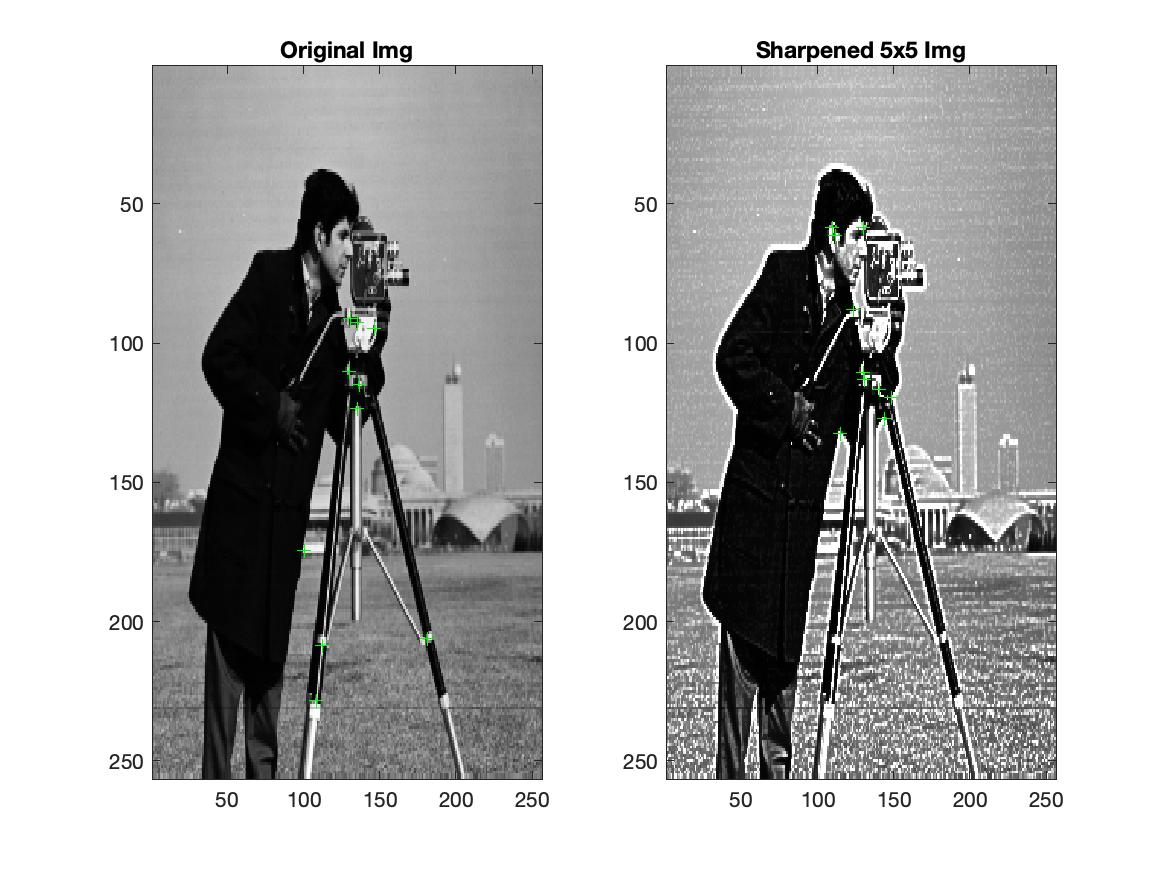
\includegraphics[width=0.5\textwidth]{Q6B_sharp5_results.jpg}
		\end{centering}
		
		
		\item text3
		
		\begin{centering}
			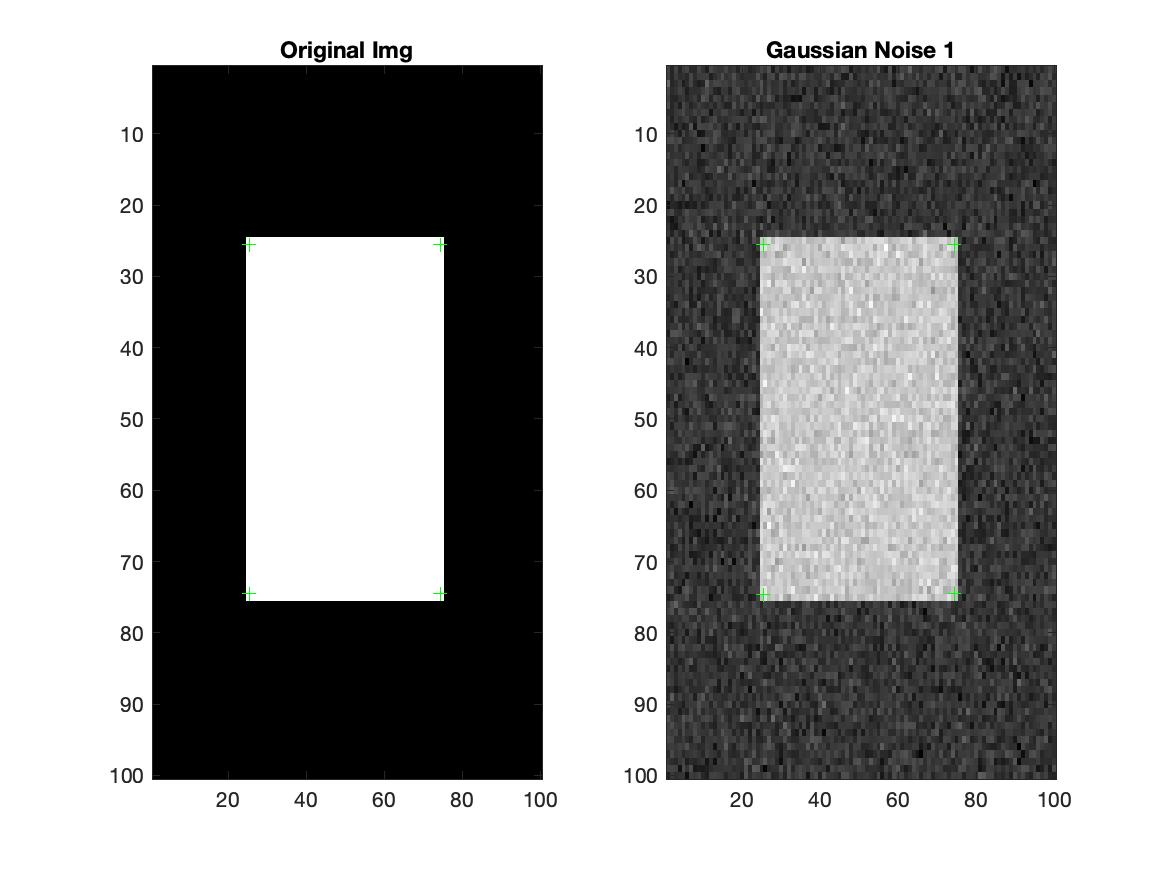
\includegraphics[width=0.5\textwidth]{Q6C_gaussian1_results.jpg}
			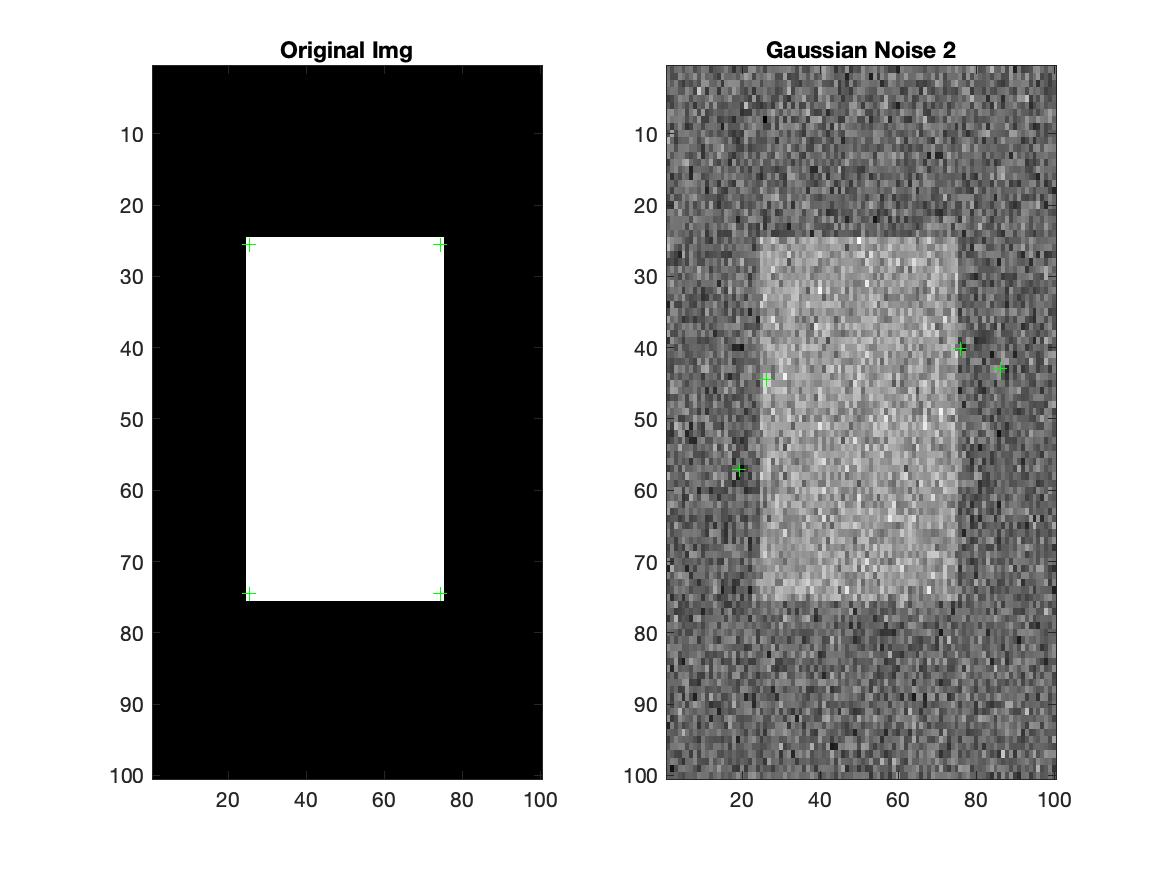
\includegraphics[width=0.5\textwidth]{Q6C_gaussian2_results.jpg}
			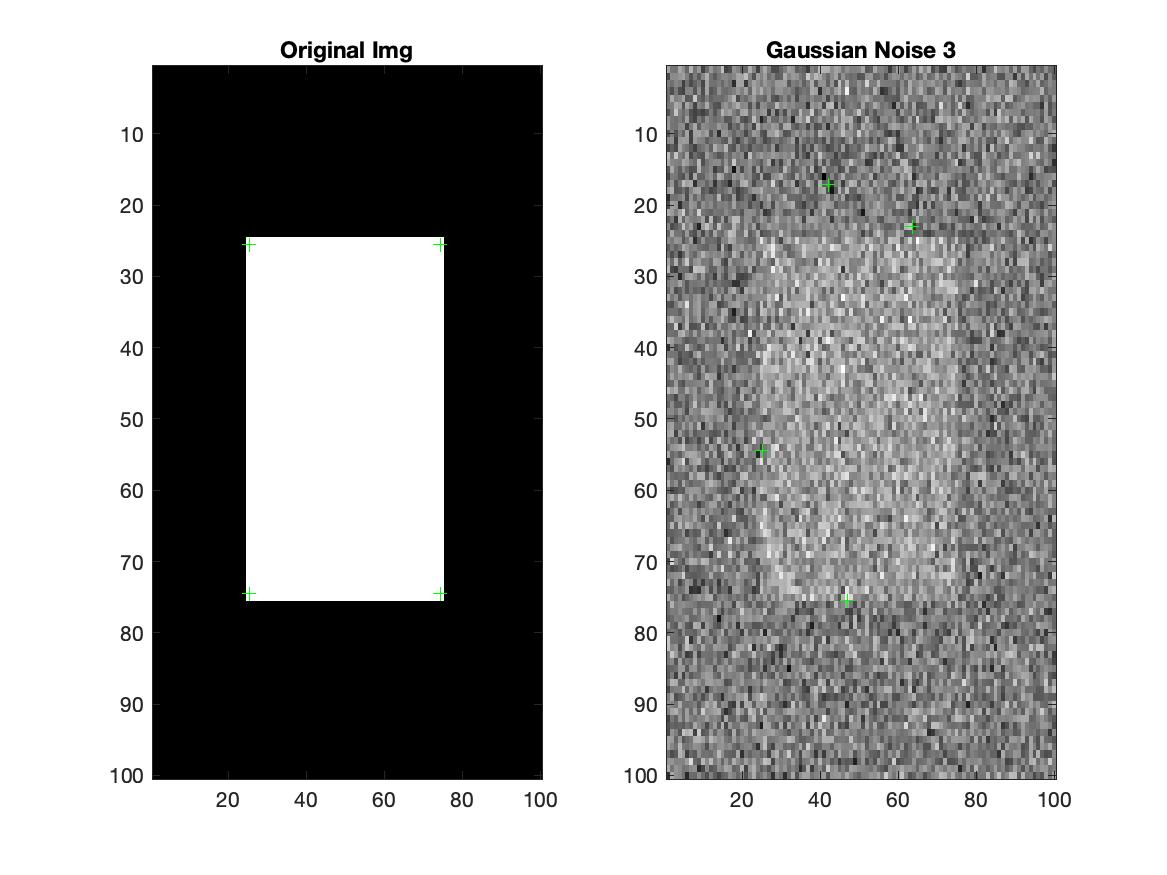
\includegraphics[width=0.5\textwidth]{Q6C_gaussian3_results.jpg}
			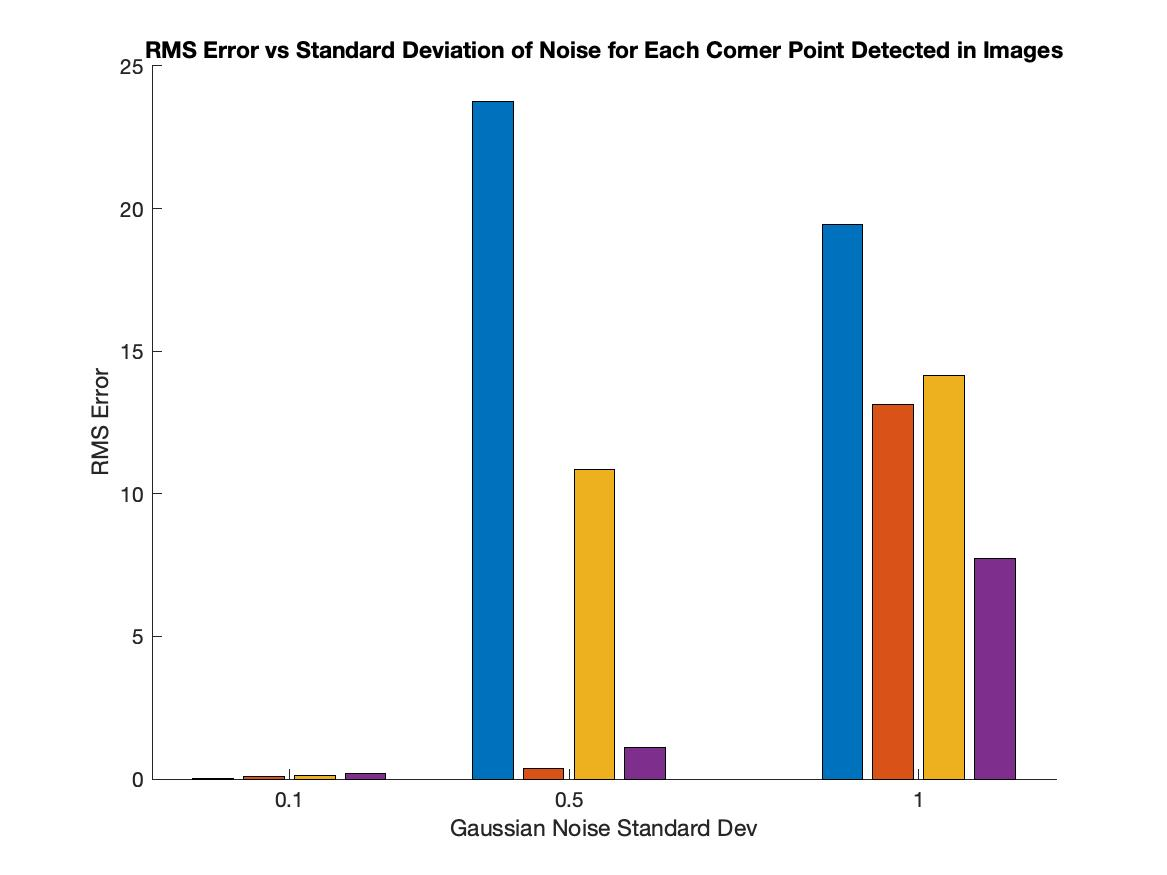
\includegraphics[width=0.5\textwidth]{Q6C_final_distribution_result.jpg}
		\end{centering}
		
		
	\end{enumerate}
\end{enumerate}
\newpage
\textbf{Matlab Code}
%\lstinputlisting{hw2.m}
\end{document}

